\documentclass[12pt,a4paper,twoside]{book}

%%%%%%%%%%%%%%%%%%%%%%%%%%%%%%%%%%%%%%%%%%%%%%%%%%%%%%%%%%%%%%%%%%%%%%%%
%%%%%%%%%%%% Packages %%%%%%%%%%%%%%%%%%%%%%%%%%%%%%%%%%%%%%%%%%%%%%%%%%
%%%%%%%%%%%%%%%%%%%%%%%%%%%%%%%%%%%%%%%%%%%%%%%%%%%%%%%%%%%%%%%%%%%%%%%%

%%%%%%
% In general useful packages
%%%%%%
\usepackage[latin1]{inputenc} % allow Umlauts
\usepackage[T1]{fontenc} % Umlauts as character in font
\usepackage{fancyhdr}   % Header/Footer
\usepackage[pdftex]{graphicx}
\usepackage{amsmath, amsthm, amssymb, amsfonts}

%%%%%%
% The following packages are optional, uncomment them if useful and required
%%%%%%
\usepackage{fancyvrb}   % extended verbatim environment
% \usepackage{latexsym}   % additional symbols
% \usepackage{times}      % bessere Schrift in PS-Dateien
% \usepackage{longtable}  % long tables (with page breaks)
% \usepackage{breakcites}  % linebreaks in cites

\usepackage[us]{datetime} % date in \today as "Month DD, YYYY", e.g., "February 29, 2012"


%%%%%%
% Hyperlinks in PDF output (blue borders, text color unchanged)
%%%%%%
\usepackage[plainpages=false, pdfpagelabels, bookmarks,  colorlinks=false,
               linkbordercolor={0 0 1}, filebordercolor={0 0 1}, citebordercolor={0 0 1},
               menubordercolor={0 0 1}, urlbordercolor={0 0 1}]{hyperref}

%%%%%%
% Another set of useful packages
%%%%%%
% \usepackage[square]{natbib}  % more powerful and customizable references
% \usepackage[center]{caption} % centered, multi-line captions of figures and tables
% \usepackage{floatflt}        % floats (e.g., figures & tables) which can have floating text around them
% \usepackage[thmmarks]{ntheorem}    % extended theorem environment
\usepackage{pdfcomment}  % comments in text as PDF notes

%%%%%%%%%%%%%%%%%%%%%%%%%%%%%%%%%%%%%%%%%%%%%%%%%%%%%%%%%%%%%%%%%%%%%%%%
%%%%%%%%%%%% Layout %%%%%%%%%%%%%%%%%%%%%%%%%%%%%%%%%%%%%%%%%%%%%%%%%%
%%%%%%%%%%%%%%%%%%%%%%%%%%%%%%%%%%%%%%%%%%%%%%%%%%%%%%%%%%%%%%%%%%%%%%%%
% German style (no paragraph indent, but gap between paragraphs)
 \setlength{\parindent}{0mm}
% \setlength{\parskip}{4pt plus3pt minus2pt}

% Page width and margins (usually no need to change, just use a4wide package)
% \setlength{\textwidth}{15cm}
% \addtolength{\oddsidemargin}{1mm}
% \addtolength{\evensidemargin}{-13.5mm}
\usepackage{a4wide} % better than individual setup

% For fancyhdr, otherwise it might result in "overfull vbox"
\addtolength{\headheight}{3.5pt}

% URL Prefix for Bibliography (i.e., no prefix, typewriter as font for URLs)
\newcommand{\urlprefix}{}
\def\UrlFont{\small\tt}
%\urlstyle{rm} % oder sf, falls obiges nicht funktioniert


%%%%%%%%%%%%%%%%%%%%%%%%%%%%%%%%%%%%%%%%%%%%%%%%%%%%%%%%%%%%%%%%%%%%%%%%
%%%%%%%%%%%% Some useful macros %%%%%%%%%%%%%%%%%%%%%%%%%%%%%%%%%%%%%%%%
%%%%%%%%%%%%%%%%%%%%%%%%%%%%%%%%%%%%%%%%%%%%%%%%%%%%%%%%%%%%%%%%%%%%%%%%

% myfigure: filename width caption
\newcommand{\myfigure}[3]{%
  \begin{figure}
    \centerline{\includegraphics[width=#2]{figures/#1.pdf}}
  \caption{#3}
  \label{fig:#1}
  \end{figure}
}

% Floating figures = figures with floating text around: filename width caption
\newcommand{\myfloatfigure}[3]{%
  \begin{floatingfigure}{#2}
    \includegraphics[width=#2]{figures/#1.pdf}
  \caption{#3}
  \label{fig:#1}
  \end{floatingfigure}
}

% two figures side by side: file1 width1 caption1 file2 width2 caption2
\newcommand{\mydoublefigure}[6]{%
  \begin{figure}
  \begin{minipage}[t]{#2}
    \centerline{\includegraphics[width=\textwidth]{figures/#1.pdf}}
  \centering
  \caption{#3}
  \label{fig:#1}
  \end{minipage}
  \hfill
  \begin{minipage}[t]{#5}
    \centerline{\includegraphics[width=\textwidth]{figures/#4.pdf}}
  \centering
  \caption{#6}
  \label{fig:#4}
  \end{minipage}
  \end{figure}
}


% Better verbatim environments (requires fancyvrb package)
\DefineVerbatimEnvironment{myverb}{Verbatim}{fontsize=\small,baselinestretch=0.84}
\DefineVerbatimEnvironment{myverbbox}{Verbatim}{frame=single,fontsize=\small,baselinestretch=0.84}


% For figures and tables
\renewcommand{\topfraction}{0.9} % a page has at most 90% of floats and at least 10% of text (if page contains floats AND text)
\renewcommand{\bottomfraction}{0.9}
\renewcommand{\floatpagefraction}{0.7} % a page with floats only is at least 70% full

% Hyphenation (include a special file with hyphenation hints if there are problems)
% \include{myhyphen}



\begin{document}

\setlength{\parindent}{2em}

\iffalse
% Title page
\begingroup
  \pagenumbering{roman}
  \thispagestyle{empty}
%\setcounter{page}{1}

%\begin{figure}
%\begin{minipage}{.4\textwidth}
\parbox{0.5cm}{\ }
   \parbox{5.1cm}{
   
\includegraphics[width=4.5cm]{rwth.jpg}}
  \parbox{2cm}{
    
\includegraphics[width=1.2cm]{i5-300.jpg}}
    \parbox{1.2cm}{\ }
  \parbox{7cm}{
    
\includegraphics[width=6cm]{iais.jpg}}  
  % \end{minipage}
%\end{figure}

\vspace*{3cm}
\centerline{{\Large\bf Computing Distributed Representations }}

\vspace*{4mm}

\centerline{{\Large\bf for Polysemous Words}}

\vspace{2cm}

\centerline{Master Thesis}
% include the title of your programme
\centerline{Software Systems Engineering}

\vspace{2cm}

\centerline{{\large Haiqing Wang}}
\centerline{Matriculation number 340863}

\vspace{10mm}

% Date!
\centerline{\today}

\vspace{10mm}

\begin{center}
\begin{minipage}[t]{8cm}
Supervisors: \\
\hspace*{2cm} Prof. Dr. Gerhard Lakemeyer \\
\hspace*{2cm} Prof. Dr. Christian Bauckhage\\[1cm]
Advisors: \\
\hspace*{2cm} Dr. Gerhard Paaß\\
\hspace*{2cm} Dr. Jörg Kindermann\\
\end{minipage}
\end{center}


\newpage

\thispagestyle{empty}

\rule{0cm}{5cm}

\newpage

\thispagestyle{empty}


\centerline{\Large{\textbf{Statutory Declaration}}}

\vspace{2cm}

\noindent I hereby certify that all work presented in this master thesis is my own,
no other than the sources and aids referred to were used and that all parts
which have been adopted either literally or in a general manner from other
sources have been indicated accordingly.


\vspace{3cm}


\begin{minipage}[t]{5cm}
Aachen, \today
\end{minipage}
\hfill
\begin{minipage}[t]{8.5cm}
\centerline{\rule{8cm}{2px}}
\centerline{YOUR NAME}
\end{minipage}

\newpage
\thispagestyle{empty}
\rule{0cm}{5cm}

%%% Include abstract and acknowledgements as necessary
\thispagestyle{empty}

\centerline{\Large{\textbf{Acknowledgements}}}

\vspace{2cm}

\noindent I would like to thank the Department of Computer Science 5 - Information Systems and Fraunhofer Institute IAIS for supporting my master thesis. I would like to express my great gratitude for the support
of Dr. Gerhard Paaß and Dr. Jörg Kindermann. Their patient guidance helps me a lot during
the research of this topic. 
\newpage
\thispagestyle{empty}

\rule{0cm}{5cm}
\thispagestyle{empty}

\centerline{\Large{\textbf{Abstract}}}

\vspace{2cm}
The inventors lack identification information and unique forms of the names for many patent offices such as the United States Patent and Trademark Office (USPTO) and the European Patent Office (EPO). Therefore, it's difficult to disambiguate the inventors with the same or similar names, and it causes troubles for the further patent analysis. This master thesis provides an automatic approach to identify the inventors. The approach creates a data structure called the inventor-patent instance to represent the patent inventor and his patents. The inventor-patent instance is described by a number of features. A global similarity between the inventor-patent instances is calculated as a weight sum of similarities based on different features. The weights and a threshold which are used for the inventor identity, are generated by using the logistic regression. Two clustering algorithms are used to group the inventor-patent instances from the same inventors in order to apply the transitivity for the inventor identity. In order to improve the clustering result, the patent-publication matching is to identify the linkages between the patent inventors and the publication authors. This master thesis report provides  the overview of the approach, describes the Java implementation and assesses its accuracy. The datasets used for the training and the testing  are two datasets from the Fleming's work \footnote{Fleming's Datasets: \url{https://dataverse.harvard.edu/dataset.xhtml? persistentId=hdl:1902.1/15705}} as well as the engineer and scientist (E\&S) dataset \footnote{E\&S Dataset : \url{http://www.patentsview.org/workshop/participants.html}} from the work done by Chunmian et al. The accuracy \footnote{The accuracy is measured mainly by the \emph{F-measure} value. The range of the \emph{F-measure} value is between 0 and 1. The larger is the value, the better is the result of the inventor identification. } of the inventor identification on the E\&S dataset is more than 0.98 while the accuracy of the inventor identification on the benchmark dataset from Fleming's research is 1.0.



%The inventors lack identification information and unique forms of names for many patent offices such as the United States Patent and Trademark Office (USPTO) and the European Patent Office (EPO). Because of that, it's difficult to disambiguate the inventors with the same or similar names. This master thesis provides an automatic approach which combines the text mining techniques, the logistic regression, the clustering and the patent-publication matching to do the inventor identification. This master thesis report provides  the overview of the approach, describes the Java implementation and assesses its accuracy. The data used for training and testing  are two datasets from the Fleming's work \footnote{Fleming's Datasets: \url{https://dataverse.harvard.edu/dataset.xhtml? persistentId=hdl:1902.1/15705}}  and the engineer and scientist (E\&S) dataset \footnote{E\&S Dataset : \url{http://www.patentsview.org/workshop/participants.html}} from the work done by Chunmian et al. The accuracy of the inventor identification on the E\&S dataset is more than 0.98 while the accuracy of the inventor identification on the benchmark dataset from Fleming's research is 1.0.



%This master thesis describes an automatic approach for the inventor identification. This approach combines the text-mining technique, the logistic regression, clustering algorithms and the patent-publication matching technique. The approach aims at making use of the available information of the patents and providing an reliable methods to disambiguate the inventors. This master thesis provides the overview of the approach, describes the Java implementation and assesses its accuracy. The evaluation of the approached is mainly based on the patent data from the United States.


\newpage
\thispagestyle{empty}
\rule{0cm}{5cm}

\newpage

\endgroup

%%%%%%%%%%%%%%%%%%%
% Header & footers
%%%%%%%%%%%%%%%%%%%

\pagestyle{fancy}

% Headers with page numbers and section/chapter titles
\renewcommand{\sectionmark}[1]{\markright{\thesection\ #1}}
\renewcommand{\chaptermark}[1]{\markboth{\thechapter\ #1}{}}
\lhead[\rm\thepage]{\sl\rightmark}
\chead{}
\rhead[\sl\leftmark]{\rm\thepage}

% Footers empty
\lfoot{}
\cfoot{}
\rfoot{}


\tableofcontents

% Include also list of figures and tables if useful
%\listoffigures
%\listoftables

\fi

%%%%%%%%%%%%%%%%%%%%
%%% Contents %%%%%%%
%%%%%%%%%%%%%%%%%%%%
% Put each chapter in a separate file


%\chapter{Introduction}
\label{cha:intro}

% Important: you have to switch to arabic numbering here!
\pagenumbering{arabic}

\begin{itemize}
\item Background / Context of the thesis
\item If applicable: describe the project the thesis is related to (e.g., CoCar)
\item Problem / Motivation
\item Goals of the thesis
\item For final thesis document: outline of the document
\end{itemize}

This is an example for a citation \cite{DBLP:journals/jods/KenscheQCJ07}.

\section{Figures}

Use vector graphics wherever possible and avoid bitmap images. Do not
use JPG at all (they are often blurred because of the compression). If
you have to include a bitmap graphics, use the PNG format. If you have
to use a JPG (as in the case for the logos on the title page), make sure
that these are images with high resolution and high quality.
\pdfcomment{pdfcomment is a useful package to put annotations like this one into the text.}

The preferred way to create a PDF image to be used in LaTeX is the following:
\begin{enumerate}
\item Do the image with your favorite graphics program (Powerpoint works well for many cases).
\item Print/Save the image as a PDF file (Acrobat Professional might be required, but
there also Open Source solutions, e.g. FreePDF)
\item Crop the image file and remove white margins.
\item Include it in LaTeX as in this example.
\end{enumerate}

How to refer to images:
Figure \ref{fig:labelOfFigure1} shows something from \cite{AfratiPODS2002}
whereas figure \ref{fig:labelOfNextFigure} is about \cite{LenzeriniPODS2002}.

If your image is not your own and taken from another source, cite the source
also in the caption.

% priority where to place the figure: here, top, bottom, page
\begin{figure}[htbp]
  % center the image.
  \centering

  % include a png file. Adapt size to 0.5 * textwidth and retain aspect ratio (!)
  \resizebox{\textwidth}{!}{
\includegraphics{Figure1.png}}

  \caption{The text under the figure \cite{AfratiPODS2002}}
  \label{fig:labelOfFigure1}
\end{figure}


\begin{figure}[htbp]
  \centering
  % Include a pdf file but make it a little smaller than the textwidth
  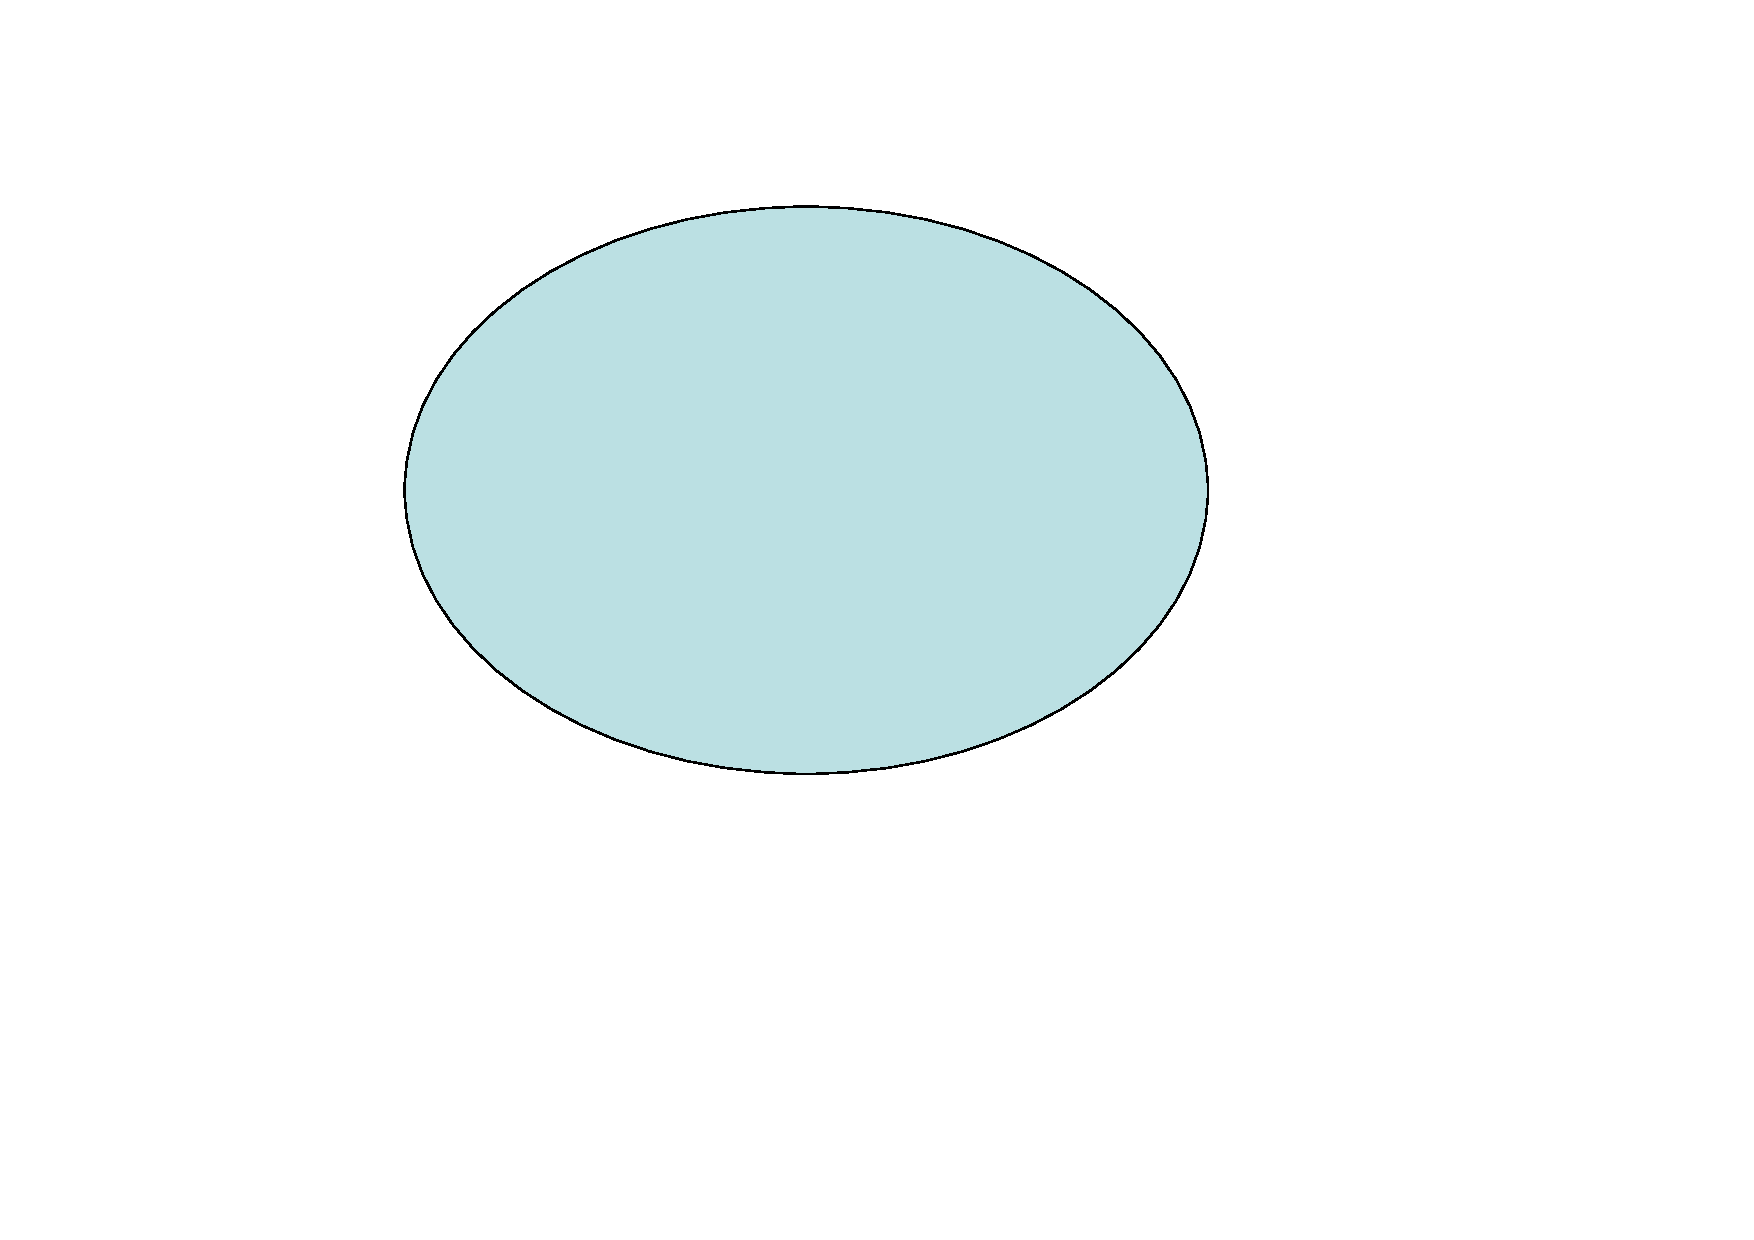
\includegraphics[width=0.5\textwidth]{Figure2.pdf}
  % Use EPS if you cannot create PDF files
  % (See http://www.wmf2eps.de.vu/ for creating eps files from powerpoint figures)
  \caption{Another text under this figure \cite{LenzeriniPODS2002}}
  \label{fig:labelOfNextFigure}
\end{figure}



%
\chapter{Related Work}
\label{cha:relwork}
This chapter introduces the related approaches for the inventor identification. These approaches can be classified into two categories. The first category is to make use of the inventor publications. In order to do that, the linkages between the inventors and the authors should be identified correctly. The second category is to leverage the information of the patent. This kind of approaches usually calculates the similarities between inventors to do the identification.


%Michele Pezzoni divides the inventor disambiguation into three steps: cleaning \& parsing, matching and filtering\cite{RePEc:grt:wpegrt:2012-29}. The cleaning \& parsing step removes the special characters from the inventor names such as punctuation, double blanks and etc. The remaining characters which are converted into ASCII codes. Then the string of the inventor name is parsed into several tokens such as surname, given name and etc. The similar process is also applied on the inventor address and the address is parsed into street, city and etc.The matching step is to match the inventors if they have a similar representation of the name. The filtering step is to decide which matching would be retained. A similarity score which is a sum of  seventeen weighted criterion is computed for each matching. The seventeen criterion could be divided into six categories: social network, geographical, applicant, technology, citation and others.  Compare this score to a threshold. If the score is larger than the threshold, the matching is retained otherwise it would be discarded.  This effectiveness of this approach is based on the quality of the data about the inventor while the clustering algorithm for my thesis is based on the contents of the patents and leverage the information of the publications which should be more robust.

\section{Identifying Author-inventors from Spain}
Maraut introduced an approach to match the inventor of the patent and the author of the publication from Spain \cite{iaifs}. The approach is divided into four steps. The first step is to struct the representations of the patents and the publications for names and addresses. The second step is to match the inventor and the author by using the names and the addresses. The address for the author is the institution address which the author is affiliated to while the addresses for the inventor are the addresses of the applicants and the inventors. The third step is to calculate a global similarity score which can be used to run a clustering to group the inventors and the authors. The inventors and the authors in the same cluster are considered as the same person. The fourth step is to control the data quality and improve the accuracy of the disambiguation manually by using recursive methods. For this approach, the weights used for the global similarity score and the threshold are calibrated manually. My approach leverages the texts of the patents and the publications to match them and identifies the weights and threshold by using the logistic regression.
%Maraut introduces an approach to match the inventor of the patent and the author of the publication from Spain\cite{iaifs}. The approach is divided into four steps. First step is to struct the name and address representations of the patents and the publications. The second step is to match the inventor and the author by using the name and the address. The address for the author is the institution address which the author is affiliated to while the addresses for the inventor are the addresses of the applicants and the inventors. The third step is to calculate a similarity global score which can be used to run a clustering to group the inventors and the authors. The inventors and the authors in the same cluster are considered as the same person. The fourth step is to control the data quality and improve the disambiguation manually by using recursive methods. For this approach, the global score is also  based on the quality of the  information about the inventor and the author. My approach would leverage the contents of the patents and the publications to match them.

\section{Measuring Industry-science Links through Inventor-author Relations: A Profiling Methodology}
Cassiman introduced a method to match the inventors of the patents and the authors of the publications based on the text-mining techniques \cite{MISLT}.  The approach first extracts the key words of the abstracts of the patents and the publications respectively.  The intersection of the sets of the keywords of the patents and the publications is used as the final term set.  A $k$-dimension vector is generated for each patent and publication respectively where $k$ is the size of the final term set. The element in the vector is the weight of a term in the document which is computed by the term frequency and the inverse document frequency.  The similarity for each pair of the patent and publication is calculated by using the cosine of the angle between the vectors. The $n$ most relevant publications  are assigned to each patent where $n$ is defined manually. The inventors of the patents and the authors of the related publications are matched if they have the same last name. Cassiman evaluated this approach by setting $n$ to 20 which resulted in a 66\% successful matching. This approach has two drawbacks. First, it generates the vectors of the documents only based on the abstracts. Second, it just computed the similarity between the publications and the patents while in my approach clustering algorithms based on the similarities between the patents are applied.  
%Cassiman introduces a method to match the inventor of the patent and author of the publication based on the text-mining techniques\cite{MISLT}.  The approach first extracts the key words of the abstract of the patents and publications respectively. Use the intersection between the sets of the keywords of the publications and patents as the final term set. Generate a $k$-dimension vector for each patent and publication respectively where $k$ is the size of the final term set. The element in the vector is the weight of a term in the document which is computed by the term frequency and inverse document frequency. Compute the similarity for each pair of the patent and publication by using the cosine of the angle between the vectors. Assign each patent the $n$ most relevant publications where $n$ is defined manually. Match the inventors of the patent and the authors of the related publications if they have the same last name. Cassiman evaluated this approach by setting $n$ to 20 which results in a 66\% successful matching. This approach have two drawbacks. First, it  generated the vectors of the documents based on the abstracts not the whole contents of the documents. Second, it just computed the similarity between the publication and patents while in my approach a clustering algorithm based on the similarity between the patents is applied which can help to distinguish the inventors with the same name. 


\section{Inventor-author Matching by Rare Name}
Kevin introduced an inventor-author matching approach based on the rare name \cite{Boyack2008173}. This approach is based on an assumption that if the inventor and the author have the same name and the name is a rare name, then they are referring to the same person. The approach calculates the rare rate for each name of the inventors and the authors. The inventor and the author are matched if they have the same name and their rare rates are bigger than a predefined threshold. This approach resulted in a 25\% matching rate. This rare name approach has some drawbacks. First, this approach can only match the inventors and the authors who are belong to the same organizations. Second, if the inventors and the authors have common names, then this approach fails to match the inventors and the authors.
%Kevin introduces an inventor-author matching approach based on the rare name. This approach is based on an assumption that if the inventor and the author have the same name and the name is a rare name, then they are referring to the same person. The approach calculates the rare rate for each name of the inventors and the authors. The rare rate of the author name is calculated as the largest percentage of the publications which belong to a certain institution. The rare rate of the inventor name is calculated in the same way but based on the information of the assignees. The inventor and the author would be matched if they have the same name and their rare rates are bigger than a predefined threshold. This approach results in a 25\% matching rate. This rare name approach has some drawbacks, first, the method doesn't match the inventor and the author in the case where the publication belongs to a institution and the patent belongs to some other organisations even if the inventor and the author are the same person. second, if the inventor and the author have a same common name, then this approach would fail to match the inventor and the author.

\section{How to Kill Inventors: Testing the Massacrator Algorithm for Inventor Disambiguation}
Pezzoni divided the inventor disambiguation into three steps: cleaning \& parsing, matching and filtering \cite{RePEc:grt:wpegrt:2012-29}. The cleaning \& parsing step removes the special characters from the inventor names such as the punctuation and double blanks. The remaining characters are converted into ASCII codes. Then the string of the inventor name is parsed into several tokens such as surname and given name. The similar process is also applied on the inventor's address and the address is parsed into the street, the city and etc. The matching step is to match the inventors if they have similar representations of the names. The filtering step is to decide which matching is retained. A similarity score which is a weight sum based on seventeen criterion is computed. The seventeen criterion are classified into six categories: social network, geography, applicant, technology, citation and others.  This score is compared to a threshold. If the score is larger than the threshold, the matching is retained and otherwise it is discarded. The weights are drawn from a uniform Bernoulli multivariate distribution while the threshold is drawn from a uniform distribution. The approach of my thesis leverages the texts of the patents and the publications of the inventors. The weights and the threshold are identified by performing the logistic regression on a training dataset. 

\section{Fleming's Inventor Disambiguation}
Fleming developed an approach by using the naive Bayesian classifier technique for the inventor disambiguation \cite{RePEc:eee:respol:v:43:y:2014:i:6:p:941-955}. The approach first selects a subset of the information from the raw patent data as features to represent the patent with a special inventor from the patent inventor list. This special form of the patent is called the inventor-patent instance. The pairs of the inventor-patent instances are the basic units for the naive Bayesian classifier. A similarity profile which contains all the similarity scores based on different features is calculated and a label is used to indicate whether the inventor-patent instances have the same inventor. The naive Bayesian classifier learns the likelihood by using a training dataset. In order to apply it on a large dataset, Fleming uses the blocking techniques by applying different criterion for each iteration. The approach creates blocks of the inventor-patent instances. The likelihood for each pair of the inventor-patent instances is used to do the agglomerative clustering until the log-likelihood reaches its maximum. 
%Fleming develops an approach by using naive Bayesian classifier technique for inventor disambiguation. The approach first selects subset of the information from the raw patent data as features to represent the patent with a special inventor from the patent inventor list. This special form of patent is called inventor-patent instance. The pairs of the inventor-patent instances are the basic units for the naive Bayesian classifier. A similarity profile which contains all the similarity score based on different feature would be calculated and a label to indicate the inventor-patent instances has the same inventor or not. The naive Bayesian classifier learn the likelihood by using this training dataset. In order to apply it to a large dataset, Fleming uses the blocking techniques, by using different criteria for each iteration. The approach creates blocks of the inventor-patent instances. Use the likelihood for each pair of the patent to do the agglomerative clustering until the log-likelihood reaches its maximum. The criterion of the blocking for each iteration would be looser and looser. 

\section{PatentsView Inventor Disambiguation Workshop}
This workshop held by the USPTO aimed at finding new approaches to solve the problem of the inventor disambiguation. There were six teams from different organizations who presented their approaches based on different techniques. This workshop provided a lot of data which can be used for the training and the testing for the participants. Thanks to the free access to these datasets, some of these datasets are also used for the training and the evaluation for my approach. Although the participants haven't published their researches' results,  their approaches are introduced according to the video and slides provided. Stephen Petrie from the Centre for Transformative Innovation (CTI) at Swinburne University of Technology introduced an approach based on the neural network of the computer vision. The approach first transforms all the information of the patents and inventors into images. Then the neural network is used to check the similarities between different images to identify the inventors.  Luciano Kay from Innovation Pulse introduced an approach based on the name comparison. The approach creates several rules to compare the inventor names. Zhen Lei from Penn State University introduced an approach based on the support vector machine. The approach not only does the inventor identification, but also builds a network based on the patent citations. Sam Ventura from Carnegie Mellon University tried to do the inventor identification based on three different techniques, the decision tree, the support vector machine and the DBSCAN.  Yang Guancan from Institute of Scientific and Technical Information of China (ISTIC) introduced an approach based on a mixture of four different techniques such as AdaBoost machine learning, stochastic record linkage, rule-based method and graph based clustering. Nicholas Monath from U Mass Amherst IESL used a word embedding technique to process the information of the patents and the hierarchical model with the inference procedure to to the inventor disambiguation. In conclusion, this workshop have shown the latest approaches for the inventor disambiguation and provided a lot of useful data. The evaluation done by the USPTO also showed us the performance of these different approaches.
%This workshop held by the USPTO aims at finding new approaches to solve the problem of the inventor disambiguation. There are six teams from different organizations who present their approaches based on different techniques. This workshop provides a lot of data which can be used for training and testing for the participants. Thanks to the free access to these datasets, some of these datasets are also used for training and evaluating my approach. Although the participants haven't published their research's result, their basic ideas of their approaches are introduced according to the video and slides provided. Stephen Petrie from the Centre for Transformative Innovation (CTI) at Swinburne University of Technology introduces an approach based on the neural network of computer vision. The approach first transforms all the information of the patents and inventors into images. Then use the neural network to check the similarities between different images to identify the inventors.  Luciano Kay from Innovation Pulse introduces an approach based on the name comparison. The approach creates several rules to compare the inventor names. Zhen Lei from Penn State University introduces an approach based on the support vector machine. The approach not only do the inventor identification, but also build a network based on the patent citation. Sam Ventura from Carnegie Mellon University tries to do the inventor identification based on three different techniques, decision tree, support vector machine and DBSCAN. The approach also tries to use the string distance to measure the similarities between the strings. Yang Guancan from Institute of Scientific and Technical Information of China (ISTIC) introduces an approach based on a mixture of four different techniques such as AdaBoost machine learning, stochastic record linkage, rule-based method and graph based clustering. Nicholas Monath from U Mass Amherst IESL uses a word embedding technique to process the information of the patents and the hierarchical model with the inference procedure to to the inventor disambiguation. In conclusion, this workshop have shown the latest approaches for the inventor disambiguation and provides a lot of useful data. The evaluation done by the USPTO also shows us the performance of different approaches.

 



%\chapter{Solution}
\label{cha:solution}

In this section we present a model for the automatic generation of embeddings for the different senses of words. Generally speaking, our model is a extension of skip-gram model with negative sampling. We assume each word in the sentence can have one or more senses. As described above  \cite{HuangSocherEtAl2012} cluster the embeddings of word contexts to label word senses and once assigned, these senses can not be changed. Our model is different. We do not assign senses to words in a preparatory step, instead we just initialize each word with random senses and they can be adjusted afterwards. We also follow the idea from EM-Algorithm based method \citep{TianDaiEtAl2014}, word's different senses have different probabilities, the probability can represent if a sense is used frequent in the corpus. 


In fact, after some experiments, we found our original model is not good. So we simplified our original model. Anyhow we will introduce our original model and show the failures in the next chapter, and explain the simplification. 

\section{Definition}

$C$ is the corpus containing \gls{M} % $M$ 
sentences, like $(S_1,S_2,\ldots,S_M)$, and each sentence is made up by several words like $S_i = (w_{i,1},w_{i,2},\ldots,w_{i,L_i})$ where $L_i$ is the length of sentence $S_i$. We use $\gls{wij} \in D$ %w_{i,j}
to represent the word token from the vocabulary $D$ in the position $j$ of sentence $S_i$. We assume that each word $w\in D$ in each sentence has $\gls{Nw}\ge1$ % $N_w$
senses.  We use the lookup function $h$ to assign senses to words in a sentence, specifically $h_{i,j}$ is the sense index of word $w_{i,j}$  ($1\leq h_{i,j}\leq N_{w_{i,j}}$). 



Similar to \cite{MikolovSutskeverEtAl2013} we use two different embeddings for the input and the output of the network.
Let $V$ and $U$ to represent respectively the set of input embedding vectors and the set of output embedding vectors respectively. And each embedding vectors has the dimension $d$. Additionally, $\gls{Vws} \in \Re^d$ % V_{w,s}
means the input embedding vectors from sense $s$ of word $w$. Similarly
$\gls{Uws} \in \Re^d$ % U_{w,s} 
is the ouput embedding of word $w$ where  $w\in D$, $1\leq s\leq N_w$. Following the Skip-gram model with negative sampling, \gls{K}. %$K$ 
The context  of a word $w_t$ in the sentence $S_i$ may be defined as the subsequence of the words  
$\gls{contextWt} = (w_{i,\max(t-c,0)},\ldots,w_{i,t-1},w_{i,t+1},\ldots,w_{i,\min(t+c,L_i)})$,  
where \gls{c} % $c$
is the size of context. And $P(w)$ 
is the smoothed unigram distribution which is used to generate negative samples. Specifically, $P(w) = \frac{count(w)^{\frac{3}{4}}}{(\sum_{i=1}^M L_i)^{\frac{3}{4}}}$ ($w\in D$), where $count(w)$ is the number of times $w$ occurred in $C$ and $\sum_{i=1}^M L_i$ is the number of total words in $C$.

\section{Objective Function}

Based on the skip-gram model with negative sampling. We still use same neural network structure to optimize the probability of using the center word to predict all words in the context. The difference is that, such probability is not about word prediction, instead it is about sense prediction. We use $(w,s)$ to represent the word $w$'s $s$-th sense, i.e. $(w_{i,t},h_{i,t})$ represents the word $w_{i,t}$'s $h_{i,t}$-th sense, and $p((w_{i,t+j},h_{i,t+j})|(w_{i,t},h_{i,t}))$ represents the probability using $w_{i,t}$'s $h_{i,t}$-th sense to predict $w_{i,t+j}$'s $h_{i,t+j}$-th sense, where $w_{i,t}$ and $w_{i,t+j}$ are indexes of words in the position $t$ and $t+j$ respectively from sentence $S_i$. And $h_{i,t}$ and $h_{i,t+j}$ represent their assigned sense indexes, which can be adjusted by model in the training. The above prediction probability is only for a pair of word with sense information, the goal of the model is to maximize every possible pairs of words which can use a probability computed by producing every prediction probabilities of word pairs to resent the prediction probability based on the whole corpus. The model's task is to adjust sense assignment and learn sense vectors in order to get the biggest prediction probability based on the whole corpus. Specifically, we use the following likelihood function to achieve above objective

\begin{equation}
\begin{split}
G = \frac{1}{M}\sum_{i=1}^M\frac{1}{L_i}\sum_{t=1}^{L_i}\sum\limits_{\mbox{\tiny$\begin{array}{c}-c\leq j \leq c\\ j\neq 0\\ 1\leq j+t\leq L_i\end{array}$}}\Bigg (\mathrm{log}\ p\Big [(w_{i,t+j},h_{i,t+j})|(w_{i,t},h_{i,t})\Big ] \\
+\sum\limits_{k=1}^K\mathbb{E}_{z_k\sim P_n(w)}\mathrm{log}\ \Big \{1-p\Big[[z_k,R(N_{z_k})]|(w_{i,t},h_{i,t})\Big ] \Big \} \Bigg )
\end{split}
\end{equation} 

where $p\Big[(w^\prime,s^\prime)|(w,s)\Big] = \sigma({U_{w^\prime,s^\prime}}^{\mathrm{T}}V_{w,s})$
 and $\sigma(x) = \frac{1}{1+\mathrm{e}^{-x}}$. 
 
 $p\Big [(w_{i,t+j},h_{i,t+j})|(w_{i,t},h_{i,t})\Big ]$ is the probability of using center word $w_{i,t}$ with sense $h_{i,t}$ to predict one surrounding word $w_{i,t+j}$ with sense $h_{i,t+j}$, which needs to be \textbf{maximized}.
$[z_1,R(N_{z_1})]$,\ldots,$[(z_K,R(N_{z_K})]$ are the negative sample words with random assigned senses to replace $(w_{i,t+j},h_{i,t+j})$, and $p\Big[[z_k,R(N_{z_k})]|(w_{i,t},h_{i,t})\Big ]\ (1\leq k\leq K)$ is the probability of using center word $w_{i,t}$ with sense $h_{i,t}$ to predict one negative sample word $z_k$ with sense $R(N_{z_k})$, which needs to be \textbf{minimized}. 
It is noteworthy that, $h_{i,t}$  ($w_{i,t}$'s sense) and $h_{i,t+j}$ ($w_{i,t+j}$'s sense) are assigned advance and $h_{i,t}$ may be changed in the \textbf{Assign}. But $z_k$'s sense $s_k$ is always assigned randomly. 

The final objective is to find out optimized parameters $\theta = \{h,U,V\}$ to maximize the Objective Function $G$, where $h$ is updated in the \textbf{Assign} and $\{U,V\}$ is updated in the \textbf{Learn}.

In the \textbf{Assign}, we use \textbf{score function} $f_{i,t}$ with fixed negative samples\\
 $\displaystyle{\mathop{\cup}_{\mbox{\tiny$\begin{array}{c}-c\leq j \leq c\\ j\neq 0\\ 1\leq j+t\leq L_i\end{array}$}}}[(z_{j,1},s_{j,1}),\ldots,(z_{j,K},s_{j,K})]$ \ (senses are assigned randomly already)
$$f_{i,t}(s) = \sum\limits_{\mbox{\tiny$\begin{array}{c}-c\leq j \leq c\\ j\neq 0\\ 1\leq t+j\leq L_i\end{array}$}}\Bigg (\mathrm{log}\ p[(w_{i,t+j},h_{i,t+j})|(w_{i,t},s) ]+\sum\limits_{k=1}^K\mathrm{log}\ \Big \{1-p[(z_{j,k},s_{j,k})|(w_{i,t},s)] \Big \} \Bigg )$$ 
to select the "best" sense (with the max value) for word $w_{i,t}$. 
In the \textbf{Learn}, we take $[ (w_{i,t},h_{i,t}),(w_{i,t+j},h_{i,t+j})]$ as a training sample and use the negative log probability as \textbf{loss function} $loss$ for each sample 
$$loss\big ( (w_{i,t},h_{i,t}),(w_{i,t+j},h_{i,t+j})\big )$$
$$ = -\mathrm{log}\ p\Big [(w_{i,t+j},h_{i,t+j})|(w_{i,t},h_{i,t})\Big ]-\sum\limits_{k=1}^K\mathbb{E}_{z_k\sim P_n(w)}\mathrm{log}\ \Big \{1-p\Big[[z_k,R(N_{z_k})]|(w_{i,t},h_{i,t})\Big ] \Big \}$$ 

And the loss function of whole corpus is $$loss(C)=\frac{1}{M}\sum_{i=1}^M\frac{1}{L_i}\sum_{t=1}^{L_i}\sum\limits_{\mbox{\tiny$\begin{array}{c}-c\leq j \leq c\\ j\neq 0\\ 1\leq j+t\leq L_i\end{array}$}}loss\big ( (w_{i,t},h_{i,t}),(w_{i,t+j},h_{i,t+j})\big )$$

	After \textbf{Assign}, $h$ is fixed. So we the same method in the normal Skip-gram with negative sampling model (stochastic gradient decent) to minimize $G$ in the \textbf{Learn}. So the objective of \textbf{Learn} is to get 
	$$\arg\min_{\{V,U\}} \frac{1}{M}\sum_{i=1}^M\frac{1}{L_i}\sum_{t=1}^{L_i}\sum\limits_{\mbox{\tiny$\begin{array}{c}-c\leq j \leq c\\ j\neq 0\\ 1\leq j+t\leq L_i\end{array}$}}loss\big ( (w_{i,t},h_{i,t}),(w_{i,t+j},h_{i,t+j})\big )$$



\section{Algorithm Description}

In the beginning, in each word of each sentence, senses are assigned \textbf{randomly}, that is $h_{i,j}$ is set to any value between $1$ to $N_{w_{i,j}}$. $N_{w_{i,j}}$ can be decide by the count of word in corpus. If the count is much, the max number of senses would be much as well. Every sense have both input embedding and output embedding, although the final experiment results shows that output embedding should have only one sense.\\

The training algorithm is an iterating between \textbf{Assign} and \textbf{Learn}. The \textbf{Assign} is to use the \textbf{score function} (sum of log probability) to select the best sense of the center word. And it uses above process to adjust senses of whole sentence and repeats that until sense assignment of the sentence is stable (not changed). The \textbf{Learn} is to use the new sense assignment of each sentence and the gradient of the \textbf{loss function} to update the input embedding and output embedding of each sense (using stochastic gradient decent). 

\paragraph{Initialization}\ \\
Input embedding vectors and output embedding vectors will be initialized from the normal Skip-gram model, which can be some public trained word vectors dataset. But in the next chapter, our experiment actually always do two steps. The first step is like normal skip-gram model and all words have only one sense. After that , the second step will use the result from that to initialize . Specifically, we use word embedding vectors from normal skip-gram model pluses some small random value (vector) to be their sense embedding vectors. Of course for different senses of the same word, the random values (vectors) are different. So in the beginning, sense vectors of each word are different but similar.


\paragraph{Sense Probabilities}\ \\
Each word has several senses. Each sense has a probability, in initialization they are set equally. For each assignment part, the probability will change based on the number of selected. Notice that , EM-Algorithm also uses sense probabilities. But our purpose to use sense probability is different. In their model, each frequent word has several senses in the meantime  with different probabilities, and in each iteration they will update the probabilities and all sense embedding vectors. While in our model, in each iteration, each word can only have one sense which can be adjusted, and after \textbf{Assign}, we only update the assigned sense. But we still use sense probabilities. The usefulness is also about recording the sense frequency, that is the assigned frequency. Some senses are selected in the \textbf{Assign}, their relative probabilities will increase. Correspondingly, for other senses which are not selected, their probabilities will decrease. 

Actually, these sense probabilities are not just used to record the assigned frequency. If some sense's probability is too low, we will use some frequent sense (assigned frequently) to reset this sense with some small random value (vector) as the same operation in the initialization. Otherwise, the infrequent assigned senses in the early iterations will always be ignored in the next iterations. Actually, we already did some experiments without sense probabilities and these experiments' results really told use the above situation. \\


Next, we will describe the specific steps of \textbf{Assign} and \textbf{Learn} in the form of pseudo-code.

\subparagraph{}\

\begin{algorithmic}
\Procedure{Assign}{}
	\For{$i$:= 1 TO $M$} \Comment{Loop over sentences.}
  \Repeat 
  \For{$t$:= 1 TO $L_i$} \Comment{Loop over words.}
\State $h_{i,t} = \max\limits_{1\leq s\leq N_{w_{i,t}}} f_{i,t}(s)$ 
  \EndFor
  \Until{no $h_{i,t}$ changed}
	\EndFor
\EndProcedure
	
\end{algorithmic}

\subparagraph{}\

\begin{algorithmic}
\Procedure{Learn}{}
\For{$i$:= 1 TO $M$} \Comment{Loop over sentences.}
	\For{$t$:= 1 TO $L_i$}  \Comment{Loop over words.}
		\For{FOR $j$:= $-c$ TO $c$}
			    \If {$j\neq 0$ \textbf{and} $t+j\geq1$ \textbf{and} $t+j\leq L_i$}
        				\State generate negative samples $\big [(z_1,s_1),\ldots,(z_K,s_K)\big ]$
        				\State $\Delta = -\nabla_\theta loss\big ( (w_{i,t},h_{i,t}),(w_{i,t+j},h_{i,t+j})\big )$
        				\State $\Delta$ is made up by $ \{\Delta_{V_{w_{i,t},h_{i,t}}}, \Delta_{U_{w_{i,t+j},h_{i,t+j}}}, [\Delta_{U_{w_1,w_1}},\ldots,\Delta_{U_{z_k,z_k}}]\}$
        				\State $V_{w_{i,t},h_{i,t}} = V_{w_{i,t},h_{i,t}} + \alpha \Delta_{V_{w_{i,t},h_{i,t}}}$
        				\State $U_{w_{i,t+j},h_{i,t+j}} = U_{w_{i,t+j},h_{i,t+j}} + \alpha \Delta_{U_{w_{i,t+j},h_{i,t+j}}}$ 
        				\State $U_{z_k,s_k} = U_{z_k,s_k} + \alpha \Delta_{U_{z_k,s_k}}, 1\leq k\leq K$ 
    				\EndIf
		\EndFor
	\EndFor			
\EndFor			
\EndProcedure
\end{algorithmic}			

\subparagraph{}\

The detail of gradient calculation of $loss\big ( (w_{i,t},h_{i,t}),(w_{i,t+j},h_{i,t+j})\big )$ is
$$\Delta_{V_{w_{i,t},h_{i,t}}} = -\frac{\partial loss\big ( (w_{i,t},h_{i,t}),(w_{i,t+j},h_{i,t+j})\big )}{\partial V_{w_{i,t},h_{i,t}}} $$
$$= [1-\mathrm{log}\ \sigma({U_{w_{i,t+j},h_{i,t+j}}}^{\mathrm{T}}V_{w_{i,t},h_{i,t}})]
U_{w_{i,t+j},h_{i,t+j}}+\sum_{k=1}^K [-\mathrm{log}\ \sigma({U_{z_k,s_k}}^{\mathrm{T}}V_{w_{i,t},h_{i,t}}))]U_{z_k,s_k}$$

$$\Delta_{U_{w_{i,t+j},h_{i,t+j}}} = -\frac{\partial loss\big ( (w_{i,t},h_{i,t}),(w_{i,t+j},h_{i,t+j})\big )}{\partial U_{w_{i,t+j},h_{i,t+j}}}$$
$$=[1-\mathrm{log}\ \sigma({U_{w_{i,t+j},h_{i,t+j}}}^{\mathrm{T}}V_{w_{i,t},h_{i,t}})]
V_{w_{i,t},h_{i,t}}$$

$$\Delta_{U_{z_k,s_k}} = -\frac{\partial loss\big ( (w_{i,t},h_{i,t}),(w_{i,t+j},h_{i,t+j})\big )}{\partial U_{z_k,s_k}}$$
$$=[-\mathrm{log}\ \sigma({U_{z_k,s_k}}^{\mathrm{T}}V_{w_{i,t},h_{i,t}}))]V_{w_{i,t},h_{i,t}}$$


\paragraph{}
Iterating between \textbf{Assign} and \textbf{Learn} till the convergence of the value of $G$ makes the whole algorithm complete. Actually, we use the loss of validation set to monitor if the training process is convergence. After a couple of iterations, we do the similar \textbf{Assign} operation on validation set and then calculate the loss. To be noted that, the \textbf{Assign} on validation set is a little different from the one on training set. Here, the negative samples needs to be always fixed throughout the training process. Another thing is that validation set and training set should not be overlapped. As long as the validation loss begin to increase.  We stop training. And select the result with best validation loss as the final result. 



%\chapter{Implementation}
\label{cha:implementation}

For the implementation of our algorithm, we use the distributed framework Apache Spark\footnote{http://spark.apache.org/}. In this chapter, we will firstly introduce some knowledge about spark and how we use these techniques to implement our model. After that, we will introduce the experiments we did and analysis our results.


\section{Introduction of Spark}


Spark was developed by \cite{ZahariaChowdhuryEtAl2010} and has many useful features for the parallel execution of programs. As the basic datastructure it has the 
\gls{RDD} % RDD
(Resilient Distributed Dataset). The RDD is a special data structure containing the items of a dataset, e.g. sentences or documents. Spark automatically distributes these items over a cluster of compute nodes and manages its physical storage. 

Spark has one driver and several executors. Usually, an executor is a cpu core, and we call each machine as worker, so each worker has several executors. But logically we only need the driver and the executors, only for something about tuning we should care about the worker stuff, e.g. some operations need to do communication between different machines. But for most of cases, each executor just fetches part of data and deals with it, and then the driver collects data from all executors.

The Spark operations can be called from different programming languages, e.g. Python, Scala, Java, and R. For this thesis we use Scala to control the execution of Spark and to define its operations.

Firstly, Spark reads text file from file system (e.g. from the unix file system or from HDFS, the Hadoop file system) and creates an RDD. An RDD usually is located in the RAM storage of the different executors, but it may also stored on (persisted to) disks of the executors. Spark operations follow the functional programming approach. There are two types of operations on RDDs: \emph{Transformation operations} and \emph{action operations}.  A transformation operation transforms  a RDD to another RDD. Examples of transformation operations are map (apply a function to all RDD elements), filter (select a subset of RDD elements by some criterion), or sort (sort the RDD items by some key). Note that an RDD is not mutable, i.e. cannot be changed. If its element are changed a new RDD is created. 

Generally after some transformation operations, people use action operations to gain some useful information from the RDD. Examples of action operations are count (count the number of items), reduce (apply a single summation-like function), aggregate (apply several summation-like functions), and collect (convert an RDD to a local array). 
 


\section{Implementation}

We use $syn0$ to represent the input embedding $V$ and $syn1$ to represent the output embedding $U$. $syn0$ and $syn1$ are defined as broadcast variables, which are only readable and can not be changed by executors. When they are changed in a training step copies are returned as a new RDD. 

\paragraph{Gradient Checking}\

Firstly we set a very small dataset mutually and calculate empirical derivative computed by the finite difference approaximation derivatives and the derivative computed as our model shows from last chapter. The result shows the difference between these two derivative is very small. So our gradient calculation is correct.\com{added (new paragraph)}

\paragraph{Data preparing} \

We use the same corpus as other papers used, a snapshot of Wikipedia at April, 2010 created by \cite{Shaoul2010}, which has 990 million tokens. Firstly we count the all words in the corpus. We transform all words to lower capital and then generate our vocabulary (dictionary). And then we calculate the frequency of word count. For example, there are 300 words which appear 10 times in the corpus. So the frequency of count 10 is 300. From this we can calculate the accumulated frequency. That is, if the accumulated frequency of count 200 is 100000, there would be 100000 words whose count is at least 200. This accumulated frequency can be used to select a vocabulary $D$ with the desired number of entries, which all appear more frequent than $minCount$ times in the corpus.  If the count of a word is smaller than $minCount$ we remove it from corpus, so it won't be in the vocabulary.  The following 4 figures (Figure \ref{fig:1to51},Figure \ref{fig:51to637},Figure \ref{fig:637to31140} and Figure \ref{fig:31140torest}) show the relationship between accumulated frequency and word count. To make visualization more clear, we display it as four different figures with different ranges of word count. And with some experience from other papers (\citep{HuangSocherEtAl2012}, \citep{TianDaiEtAl2014} and \citep{NeelakantanShankarEtAl2015}), in some of our experiments we set $minCount=20$ and others have $minCount=200$. Actually, when word count is 20, the accumulated frequency is 458142, that is the vocabulary size would be 458142; when word count is 200, the accumulated frequency is 95434, that is the vocabulary size would be 95434.


\begin{figure}[H]
\centering
    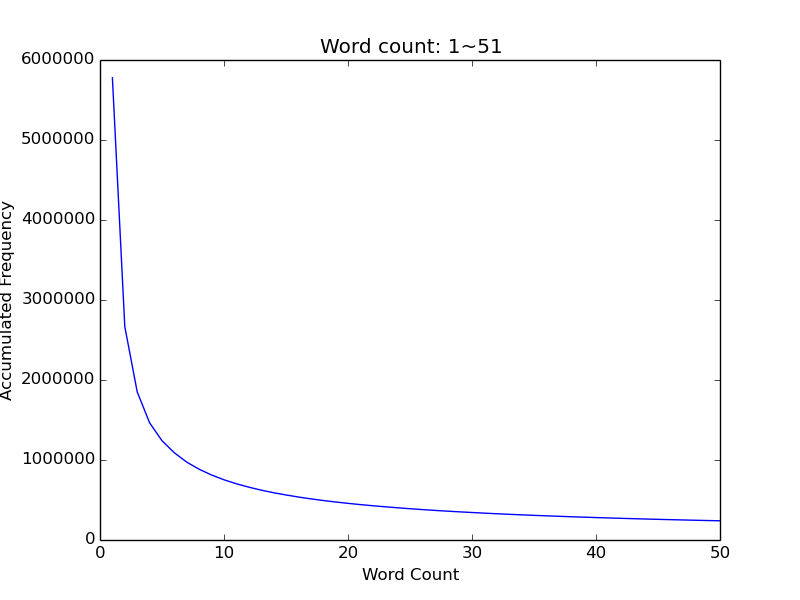
\includegraphics[width=0.75\textwidth]{1to51} 
	\caption{Shows the accumulated frequency of word count in range [1,51]}
	\label{fig:1to51}
\begin{figure}[H]
\centering
  \end{figure}
        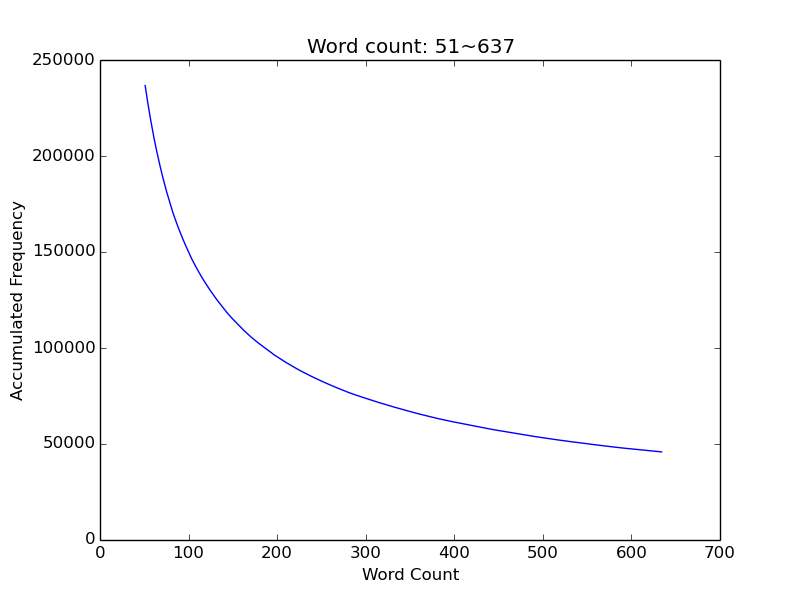
\includegraphics[width=0.75\textwidth]{51to637} 
	\caption{Shows the accumulated frequency of word count in range [51,637]}
	\label{fig:51to637}
\end{figure}


\begin{figure}[H]
\centering
 	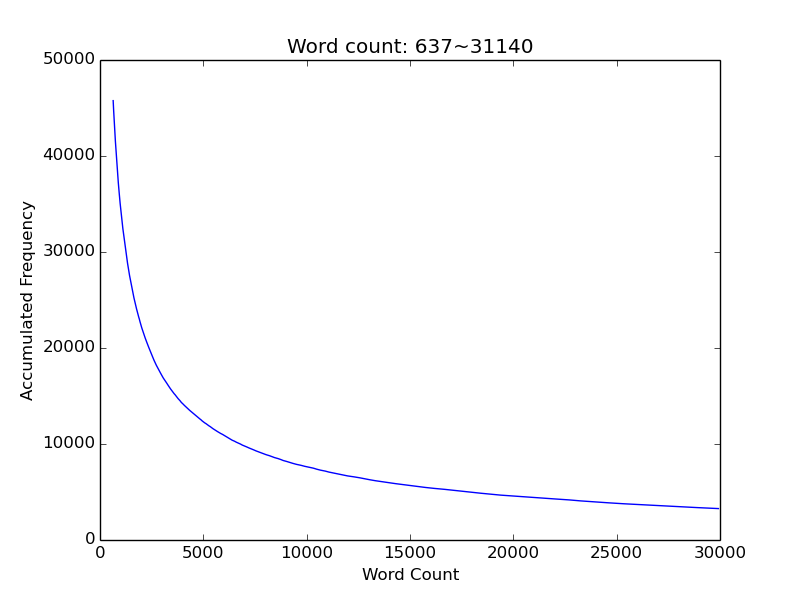
\includegraphics[width=0.75\textwidth]{637to31140} 
	\caption{Shows the accumulated frequency of word count in range [637,31140]}
	\label{fig:637to31140}
\begin{figure}[H]	
\end{figure}
\centering
	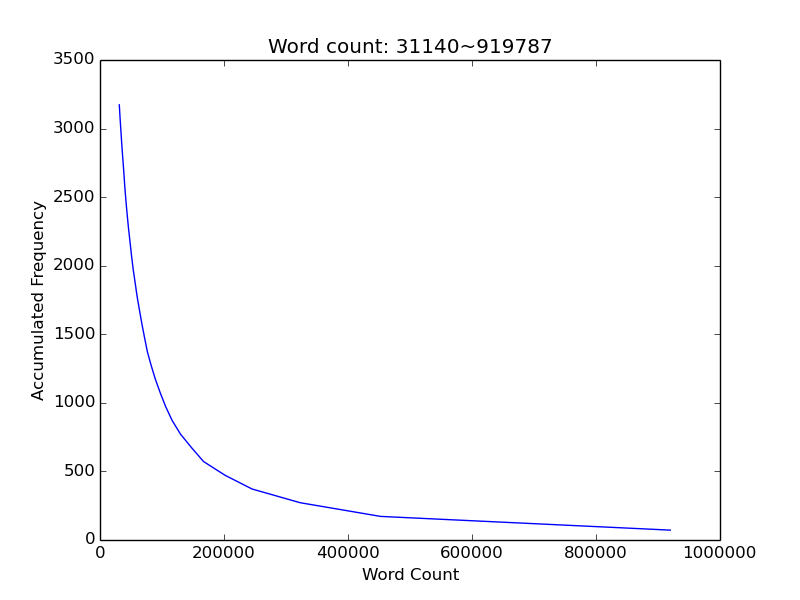
\includegraphics[width=0.75\textwidth]{31140torest} 
	\caption{Shows the accumulated frequency of word count in range [637,919787]}
	\label{fig:31140torest}
\end{figure}

\paragraph{Computing Environment} \ 

Our program is running on a single machine with 32 cores. For some experiments, we use all cores as executers. We also tried some experiments on a compute cluster of several machines, but the time of collecting parameters ($syn0$ and$syn1$) is too slow and actually too many executors actually is not really good for our program. After learning parameters parallel by stochastic gradient, the program collects all parameters and calculates the average, which reduces the learning effect and slow down the convergence especial when the number of executors is too many, although more executors can speed up training more or less. \del{We also tried some experiments on a compute cluster of several machines, but that is not very good for our program, we will explain some reasons later. So there is no communication between different machines.  But there are some experiments requiring fewer cores.}


\paragraph{Training set and validation set} \ 

We split the corpus into a training set and a validation set. The training set has $99\%$ of the data and validation set has only $1\%$ of the data. We use the validation set to monitor our training process if it is converging. If the training algorithm  converges, the loss of validation set should be at the lowest value. And then it gradually increases, which means the training is over-fitting. So we calculate the loss of the validation set after several training iterations and then compare with the previous validation loss. If the current value is bigger than previous value, we stop our training process and fetch the previous result as the final result to store to the disk. That is, after each calculation of the loss of validation set, we store our results. 

Note that, the validation set and training set should not be overlapping, because we use the validation set to monitor our training. And another import thing is that, the negative samples of validation set should always be fixed to reduce variance.  The assignment step for the word senses of the validation set is almost the same as the one for training set. The only different thing is that the negative samples for each word of each sentence in the validation set are not changed. But for each iteration of sense assignment for sentences in the training set, the negative sampling are new. 


Another thing is that, for each iteration, we do not use the whole training set to assign senses and learn parameters. Instead we split the training set into several parts and each time we only fetch one data part to do sense assignment (Assign Step)and parameters learning (Learn Step). Specifically, the training set was split into $numRDD$ different RDDs, which were persisted to disk to allow execution of the training in RAM. $numRDD$ is the number of RDD to split training dataset.

\paragraph{Learning Rate Reduction}\

At the beginning of experiment, the learning rate is set to $lr$. After each iteration, the learning rate will be reduced with a reduction factor $gm$. Specifically, using $\alpha$ to represent current learning rate and $\alpha^\prime$ to represent the new learning rate, we have
$$\alpha^\prime=\alpha*gm$$

\paragraph{Iteration}\ 

As described before, the while training process include several iterations. At the beginning the program fetches the first RDD and then for next each iteration, the it fetches one of other RDDs orderly. After several iterations, the program finishes processing all RDDs, and for the next iteration (if not stopping) it will fetches the first RDD again and repeat the above . Each iteration contains the sense assignment, adjusting the sense probabilities for each word based on the assigned senses, learning parameters , collecting parameters using $treeAggregate$ and normalizing sense embeddings, and every operations are on training set. And in some iteration (not every), the program assigns senses on the validation set and stores the RDD data. In experiments we compare the time of each operation in an iteration, and find that comparing the time of learning parameters and the time of parameters collection, the time of other operations can be ignored. Define $t1$ as the average time of learning parameters in an iteration, $t2$ as the collecting parameters in an iteration, $t3$ as the average time of all operations in an iteration, $t4$ as the total training time and $iter$ as the total number of iterations. And we will do some analysis on these time in next chapter.

\com{changed}

\paragraph{Assign Step}\ \\
In the assignment, we use map transformation to transform each sentence with senses information to another sentence with changed senses information. The sense with the lowes loss is selected. So one RDD is transformed to another RDD. In this process, $syn0$ and $syn1$ are constant and will be used (only read) to calculate the loss. 


\paragraph{Learn Step}\ \\
In the training, we also use a map transformation. Instead of transforming sentences to sentences, we transform the original sentence RDD into the two-element collection of the updated $syn0$ and updated $syn1$. We broadcast these variables to the local $syn0$ and $syn1$ in each executor, so that each executor has its own  copy of $syn0$ and $syn1$ and can update them independently. So each executor has copies of $syn0$ and $syn1$. And then we use $treeAggregate$ to collect all such vectors together from different executors (cpu cores).  In the aggregation operation, different $syn0$'s vectors add up together, and different $syn0$'s vectors add up together. Finally, by dividing by the the number of partitions, we get one global $syn0$ and one global $syn1$ in the driver. For now, we set them as new $syn0$ and $syn1$, which will be broadcasted again in the next iteration. 

\paragraph{Normalization}\ \\
After getting the new global $syn0$ and $syn1$, some values of some embeddings may be very big. Thus, we need to do normalization to avoid to big values. Our normalization method is very simple, which is to check all embeddings from $syn0$ and $syn1$ if their Euclidean length is bigger than 4. If that is the case we just normalize them to the new embeddings with length of 4.



%\chapter{Evaluation}
\label{cha:eval}

\begin{itemize}
\item In the proposal: describe the data sets and measures which you plan
      to use in the evaluation. Make sure that the resources (data, users, etc.)
      which are required for the evaluation are really available.
\item In the thesis: describe the data sets and measures which you have used.
      Give the results in form of diagrams (e.g., Excel or Gnuplot). Discuss
      different variants of your solutions and different parameter settings.
      If available, compare your results with an existing approach. Important:
      Also negative results are results: ``The approach did not work for this
      data set because ...'' This is important information, because nobody wants
      to do again the same experiments as you already did. In case of performance
      numbers, give a detailed description of the hardware which was used to do
      the experiments. Discuss the results (what is good, what is bad).
\end{itemize}

%\chapter{Conclusion}
\label{cha:concl}

My master thesis provides an approach for the inventor identification by using clustering algorithms combined with the logistic regression and the patent-publication matching. The approach first extends the Fleming's inventor-patent instance data structure by adding four text features. Different methods are designed to calculate the similarities based on different features. With a training dataset, the approach uses the logistic regression to assign each feature similarity a suitable weight and find a suitable threshold to decide if two inventor-patent instances are from the same inventor. The DBSCAN and the hierarchical clustering try to group the inventor-patent instances from the same inventor and perform the transitivity for the inventor identity. The clustering algorithms make use of the weights and the threshold generated by the logistic regression. Some optimization techniques such as LSI, the "Bold-driver" technique and the "Stop-early" technique are used for optimizations. From the evaluation result, the clustering algorithms combined with the logistic regression show good performances for the inventor identification. Because of the good performances of clustering algorithms and the incomplete information provided by the publication database, the patent-publication matching doesn't help to improve the accuracy. In conclusion, the approach has a good ability to do the inventor identification.
\newline

There are several directions for the future work. If the approach is going to be applied on another patent database, a representative training dataset should be prepared for the logistic regression. The training dataset is generated from the inventor-patent instance dataset which contains $\frac{n(n-1)}{2}$ pieces of data where $n$ is the number of inventor-patent instances. Some techniques such as the mini-batch gradient descent method or the stochastic gradient descent method can be used to accelerate the training process when the size of the training dataset becomes large. From the evaluation, the single linkage clustering and the minPts with 1 show the best performances. Both of them make the transitivity into a high level. The transitivity as a high level aims at decreasing the \emph{splitting} error. But in the future, more and more inventors would have the same name. Keeping the transitivity as a high level may result in a bigger \emph{lumping} error. Except finding a better training dataset, the method to calculate the similarities between clusters and the value of minPts should also be adjusted again to find the best performance. 

\newpage
\thispagestyle{empty}
\rule{0cm}{5cm}

%Although the patent-publication matching doesn't help to improve the accuracy during the evaluation process, it is still promising to be helpful if a good publication database can be found.




%%% Use appendix if necessary
% \begin{appendix}
% \chapter{Appendix}
\label{cha:appendix}
% \end{appendix}

% References
%
% There many ways to get a bibliography style
% 1. Use thesis.bst as included in this package (reasonable layout)
% 2. Customize thesis.dbj and rerun "latex thesis.dbj" to produce a new thesis.bst
%    (for experienced user)
% 3. Run "tex makebst.tex" (using makebst.tex from the custom-bib package) to create your own DBJ & BST-file
%    (for the very experienced user)
% 4. Code your BST file from scratch (for the BibTeX nerd)

% thesis.bst as included should be a good start, though
\bibliographystyle{thesis}

% Use bibtex to manage your references
% Jabref is a useful tool for editing a bibtex file
% The bibtex file modelman.bib included in this template
% is a snapshot of the main bibtex file of the group.
% The most recent version is in the CVS directory papers/bib
% In any case, give complete information about the references:
% Authors, title, place of publication (conference,journal),
% Year of publication, page numbers, URL if the document is
% also available online.
\bibliography{modelman}










\section{Skipgram-model with negative sampling}
\subsection{Introduction}

Negative sample words are sampled according to a smoothed unigram distribution.
\subsection{Definition}
\ \ \ \ \ \ Corpus $C$: $(S_1,S_2,\ldots,S_M)$

$M$: the total number of sentences\\

$S_i$: the $i$th sentence,\ \ $S_i = (w_{i,1},w_{i,2},\ldots,w_{i,L_i})$

$L_i$: the length of sentence $S_i$

$w_{i,j}$: the word in the position $j$ of sentence $S_i$\\

$V$: lookup table of sense input embedding 

$U$: lookup table of  sense output embedding 

$V_w$: the input embedding of $w$, $w\in D$, $V_w \in \mathbb{R}^d$

$U_w$: the output embedding of $w$, $w\in D$, $U_w \in \mathbb{R}^d$

$D$: Vocabulary 

$d$: the size of embedding vector (both input and output)\\

$K$: the number of negative samples\\

$R()$: a random number (real) from 0.0 to 1.0\\

$c$: the size of context\\

$P_n(w)$: smoothed unigram distribution ,\ \ $P_n(w) = \frac{count(w)^{\frac{3}{4}}}{(\sum_{i=1}^M L_i)^{\frac{3}{4}}}$, \ \ $w\in D$

$count(w)$: the number of times $w$ occurred in $C$

$\sum_{i=1}^M L_i$: the number of total words in $C$
\subsection{Objective Function}
\begin{equation}
\begin{split}
G = \frac{1}{M}\sum_{i=1}^M\frac{1}{L_i}\sum_{t=1}^{L_i}\sum\limits_{\mbox{\tiny$\begin{array}{c}-c\leq j \leq c\\ j\neq 0\\ 1\leq j+t\leq L_i\end{array}$}}\Big \{\mathrm{log}\ p(w_{i,t+j}|w_{i,t}) 
+\sum\limits_{k=1}^K\mathbb{E}_{z_k\sim P_n(w)}\mathrm{log}\ [1-p(z_k|w_{i,t}) ] \Big \}
\end{split}
\end{equation} 

where $p(w^\prime|w) = \sigma({U_{w^\prime}}^{\mathrm{T}}V_w)$
 and $\sigma(x) = \frac{1}{1+\mathrm{e}^{-x}}$.\\
 
 $p(w_{i,t+j}|w_{i,t})$ is the probability of using center word $w_{i,t}$ to predict one surrounding word $w_{i,t+j}$, which needs to be \textbf{maximized}.
$z_1$,\ldots,$z_K$ are the negative sample words to replace word $w_{i,t+j}$, and $p(z_k|w_{i,t})\ (1\leq k\leq K)$ is the probability of using center word $w_{i,t}$ to predict one negative sample word $z_k$, which needs to be \textbf{minimized}. Equivalently, the whole objective function needs to be \textbf{maximized}. \\ 

Take $(w_{i,t},w_{i,t+j})$ as a training sample, and define \textbf{loss function} $loss$ for each sample 
$$loss(w_{i,t},w_{i,t+j})$$
$$ = -\mathrm{log}\ p(w_{i,t+j}|w_{i,t})-\sum\limits_{k=1}^K\mathbb{E}_{z_k\sim P_n(w)}\mathrm{log}\ [1-p(z_k|w_{i,t})] $$
Here the loss is defined as the negative log probability. \\

	And the loss function of whole corpus is $$loss(C)=\frac{1}{M}\sum_{i=1}^M\frac{1}{L_i}\sum_{t=1}^{L_i}\sum\limits_{\mbox{\tiny$\begin{array}{c}-c\leq j \leq c\\ j\neq 0\\ 1\leq j+t\leq L_i\end{array}$}}loss(w_{i,t},w_{i,t+j})$$
	To maximize the objective function is equivalently to minimize the loss function. So the objective of learning algorithm is 
	$$\arg\min_{\{V,U\}} \frac{1}{M}\sum_{i=1}^M\frac{1}{L_i}\sum_{t=1}^{L_i}\sum\limits_{\mbox{\tiny$\begin{array}{c}-c\leq j \leq c\\ j\neq 0\\ 1\leq j+t\leq L_i\end{array}$}}loss(w_{i,t},w_{i,t+j})$$ 

	Use 
	$$N = \frac{1}{M}\sum_{i=1}^M\frac{1}{L_i}\sum_{t=1}^{L_i}\sum\limits_{\mbox{\tiny$\begin{array}{c}-c\leq j \leq c\\ j\neq 0\\ 1\leq j+t\leq L_i\end{array}$}} 1$$
	to represent the number of total training samples in one epoch. (An epoch is a measure of the number of times all of the training samples are used once.) And the number of epochs is $T$. So the total iterations is $N*T$.\\
	
	Use stochastic gradient descent: 
	\begin{itemize}
	\item Initialize $\{V,U\}$
	\item For $N*T$ Iterations: 
		\begin{itemize}
		\item For each training sample $(w_{i,t},w_{i,{t+j}})$
		\begin{itemize}
		\item Generate negative sample words to replace $w_{i,t+j}$: $(w_1,\ldots,z_k)$
		\item Calculate the gradient $\Delta = -\nabla_{\{V,U\}} loss(w_{i,t},w_{i,{t+j}})$
		\item $\Delta$ is only made up by $\{\Delta_{V_{w_{i,t}}}, \Delta_{U_{w_{i,t+j}}}, [\Delta_{U_{w_1}},\ldots,\Delta_{U_{z_k}}]\}$
		\item Update Embeddings: 
		\begin{itemize}
		\item $V_{w_{i,t}} = V_{w_{i,t}}+\alpha\Delta_{V_{w_{i,t}}}$
		\item $U_{w_{i,t+j}} = U_{w_{i,t+j}}+\alpha\Delta_{U_{w_{i,t+j}}}$
		\item $U_{z_k} = U_{z_k}+\alpha\Delta_{U_{z_k}}, 1\leq k\leq K$ 
		\end{itemize}
		($\alpha$ is the learning rate and will be updated every several iterations)
		\end{itemize}
		\end{itemize}
	\end{itemize}
The detail of gradient calculation of $loss(w_{i,t},w_{i,t+j})$ is
	$$\Delta_{V_{w_{i,t}}} = -\frac{\partial loss(w_{i,t},w_{i,t+j})}{\partial V_{w_{i,t}}} = [1-\mathrm{log}\ \sigma(U_{w_{i,t+j}}^{\mathrm{T}}V_{w_{i,t}})]U_{w_{i,t+j}}+\sum_{i=1}^k [-\mathrm{log}\ \sigma(U_{z_k}^{\mathrm{T}}V_{w_{i,t}}))]U_{z_k}$$
	$$\Delta_{U_{w_{i,t+j}}} = -\frac{\partial loss(w_{i,t},w_{i,t+j})}{\partial U_{w_{i,t+j}}} = [1-\mathrm{log}\ \sigma(U_{w_{i,t+j}}^{\mathrm{T}}V_{w_{i,t}})]V_{w_{i,t}}$$
	$$\Delta_{U_{z_k}} = -\frac{\partial loss(w_{i,t},w_{i,t+j})}{\partial U_{z_k}} = [-\mathrm{log}\ \sigma(U_{z_k}^{\mathrm{T}}V_{w_{i,t}}))]V_{w_{i,t}}, 1\leq k\leq K$$ 

\section{Sense Assignment based on SGNS}
\subsection{Introduction}
\ \ \ \ \ \ Corpus is made up by $M$ sentences, and each sentence is made up by several words. Each word in each sentence has one or multiple senses. In the beginning, in each word of each sentence, senses are assigned \textbf{randomly}. Every sense have both input embedding and output embedding.\\

The training algorithm is an iterating between \textbf{Assign} and \textbf{Learn}. The \textbf{Assign} is to use the \textbf{score function} (sum of log probability) to select the best sense of the center word. And it uses above process to adjust senses of whole sentence and repeats that until sense assignment of the sentence is stable (not changed). The \textbf{Learn} is to use the new sense assignment of each sentence and the gradient of the \textbf{loss function} to update the input embedding and output embedding of each sense (using stochastic gradient decent). 
\subsection{Definition}

\ \ \ \ \ \ Corpus $C$: $(S_1,S_2,\ldots,S_M)$

$M$: the total number of sentences\\

$S_i$: the $i$th sentence \ , \ $S_i = (w_{i,1},w_{i,2},\ldots,w_{i,L_i})$

$L_i$: the length of sentence $S_i$\\

$w_{i,j}$: the word in the position $j$ of sentence $S_i$

$h$: lookup table of sense assignment

$h_{i,j}$: the sense index of word $w_{i,j}$, \ $1\leq h_{i,j}\leq N_{w_{i,j}}$

$N_w$: the max number of senses of word $w$, \ $w\in D$\\

$V$: lookup table of sense input embedding 

$U$: lookup table of  sense output embedding 

$V_{w,s}$: the input embedding of sense $s$ of word $w$, $w\in D$, $1\leq s\leq N_w$, $V_{w,s} \in \mathbb{R}^d$

$U_{w,s}$: the output embedding of sense $s$ of word $w$, $w\in D$, $1\leq s\leq N_w$, $U_{w,s} \in \mathbb{R}^d$\\

$D$: Vocabulary 

$d$: the size of embedding vector (both input and output)\\

$K$: the number of negative samples\\

$R(x)$: a random number (integer) from 1 to $x$

$R()$: a random number (real) from 0.0 to 1.0\\

$c$: the size of context\\

$P_n(w)$: smoothed unigram distribution ,\ \ $P_n(w) = \frac{count(w)^{\frac{3}{4}}}{(\sum_{i=1}^M L_i)^{\frac{3}{4}}}$, \ \ $w\in D$

$count(w)$: the number of times $w$ occurred in $C$

$\sum_{i=1}^M L_i$: the number of total words in $C$

\subsection{Objective Function}
\begin{equation}
\begin{split}
G = \frac{1}{M}\sum_{i=1}^M\frac{1}{L_i}\sum_{t=1}^{L_i}\sum\limits_{\mbox{\tiny$\begin{array}{c}-c\leq j \leq c\\ j\neq 0\\ 1\leq j+t\leq L_i\end{array}$}}\Bigg (\mathrm{log}\ p\Big [(w_{i,t+j},h_{i,t+j})|(w_{i,t},h_{i,t})\Big ] \\
+\sum\limits_{k=1}^K\mathbb{E}_{z_k\sim P_n(w)}\mathrm{log}\ \Big \{1-p\Big[[z_k,R(N_{z_k})]|(w_{i,t},h_{i,t})\Big ] \Big \} \Bigg )
\end{split}
\end{equation} 

where $p\Big[(w^\prime,s^\prime)|(w,s)\Big] = \sigma({U_{w^\prime,s^\prime}}^{\mathrm{T}}V_{w,s})$
 and $\sigma(x) = \frac{1}{1+\mathrm{e}^{-x}}$. \\
 
 $p\Big [(w_{i,t+j},h_{i,t+j})|(w_{i,t},h_{i,t})\Big ]$ is the probability of using center word $w_{i,t}$ with sense $h_{i,t}$ to predict one surrounding word $w_{i,t+j}$ with sense $h_{i,t+j}$, which needs to be \textbf{maximized}.
$[z_1,R(N_{z_1})]$,\ldots,$[(z_K,R(N_{z_K})]$ are the negative sample words with random assigned senses to replace $(w_{i,t+j},h_{i,t+j})$, and $p\Big[[z_k,R(N_{z_k})]|(w_{i,t},h_{i,t})\Big ]\ (1\leq k\leq K)$ is the probability of using center word $w_{i,t}$ with sense $h_{i,t}$ to predict one negative sample word $z_k$ with sense $R(N_{z_k})$, which needs to be \textbf{minimized}. 
It is noteworthy that, $h_{i,t}$  ($w_{i,t}$'s sense) and $h_{i,t+j}$ ($w_{i,t+j}$'s sense) are assigned advance and $h_{i,t}$ may be changed in the \textbf{Assign}. But $z_k$'s sense $s_k$ is always assigned randomly. \\

The final objective is to find out optimized parameters $\theta = \{h,U,V\}$ to maximize the Objective Function $G$, where $h$ is updated in the \textbf{Assign} and $\{U,V\}$ is updated in the \textbf{Learn}.\\

When the center word $w_{i,t}$ is giving, we use \textbf{score function} $f_{i,t}$ with fixed negative samples $\displaystyle{\mathop{\cup}_{\mbox{\tiny$\begin{array}{c}-c\leq j \leq c\\ j\neq 0\\ 1\leq j+t\leq L_i\end{array}$}}}[(z_{j,1},s_{j,1}),\ldots,(z_{j,K},s_{j,K})]$ \ (senses are assigned randomly already)
$$f_{i,t}(s) = \sum\limits_{\mbox{\tiny$\begin{array}{c}-c\leq j \leq c\\ j\neq 0\\ 1\leq t+j\leq L_i\end{array}$}}\Bigg (\mathrm{log}\ p[(w_{i,t+j},h_{i,t+j})|(w_{i,t},s) ]+\sum\limits_{k=1}^K\mathrm{log}\ \Big \{1-p[(z_{j,k},s_{j,k})|(w_{i,t},s)] \Big \} \Bigg )$$ 
to select the "best" sense (with the max value) of each center word in the \textbf{Assign}. \\

Taking $[ (w_{i,t},h_{i,t}),(w_{i,t+j},h_{i,t+j})]$ as a training sample, we define \textbf{loss function} $loss$ for each sample as
$$loss\big ( (w_{i,t},h_{i,t}),(w_{i,t+j},h_{i,t+j})\big )$$
$$ = -\mathrm{log}\ p\Big [(w_{i,t+j},h_{i,t+j})|(w_{i,t},h_{i,t})\Big ]-\sum\limits_{k=1}^K\mathbb{E}_{z_k\sim P_n(w)}\mathrm{log}\ \Big \{1-p\Big[[z_k,R(N_{z_k})]|(w_{i,t},h_{i,t})\Big ] \Big \}$$
Here the loss is defined as the negative log probability. \\

And the loss function of whole corpus is $$loss(C)=\frac{1}{M}\sum_{i=1}^M\frac{1}{L_i}\sum_{t=1}^{L_i}\sum\limits_{\mbox{\tiny$\begin{array}{c}-c\leq j \leq c\\ j\neq 0\\ 1\leq j+t\leq L_i\end{array}$}}loss\big ( (w_{i,t},h_{i,t}),(w_{i,t+j},h_{i,t+j})\big )$$

	After \textbf{Assign}, $h$ is fixed. So we use the same method in the normal Skip-gram with negative sampling model (stochastic gradient decent) to minimize $G$ in the \textbf{Learn}. So the objective of \textbf{Learn} is 
	$$\arg\min_{\{V,U\}} \frac{1}{M}\sum_{i=1}^M\frac{1}{L_i}\sum_{t=1}^{L_i}\sum\limits_{\mbox{\tiny$\begin{array}{c}-c\leq j \leq c\\ j\neq 0\\ 1\leq j+t\leq L_i\end{array}$}}loss\big ( (w_{i,t},h_{i,t}),(w_{i,t+j},h_{i,t+j})\big )$$
	
	
Use 
	$$N = \frac{1}{M}\sum_{i=1}^M\frac{1}{L_i}\sum_{t=1}^{L_i}\sum\limits_{\mbox{\tiny$\begin{array}{c}-c\leq j \leq c\\ j\neq 0\\ 1\leq j+t\leq L_i\end{array}$}} 1$$
	to represent the number of total training samples in one epoch. (An epoch is a measure of the number of times all of the training samples are used once.) .\\
	
	Use stochastic gradient descent: 
	\begin{itemize}
	\item For $N$ Iterations: 
		\begin{itemize}
		\item For each training sample $(w_{i,t},w_{i,{t+j}})$
		\begin{itemize}
		\item Generate negative sample words to replace $w_{i,t+j}$: $(w_1,\ldots,z_k)$
		\item Calculate the gradient $\Delta = -\nabla_{\{V,U\}} loss(w_{i,t},w_{i,{t+j}})$
		\item $\Delta$ is only made up by $\{\Delta_{V_{w_{i,t}}}, \Delta_{U_{w_{i,t+j}}}, [\Delta_{U_{w_1}},\ldots,\Delta_{U_{z_k}}]\}$
		\item Update Embeddings: 
		\begin{itemize}
		\item $V_{w_{i,t}} = V_{w_{i,t}}+\alpha\Delta_{V_{w_{i,t}}}$
		\item $U_{w_{i,t+j}} = U_{w_{i,t+j}}+\alpha\Delta_{U_{w_{i,t+j}}}$
		\item $U_{z_k} = U_{z_k}+\alpha\Delta_{U_{z_k}}, 1\leq k\leq K$ 
		\end{itemize}
		($\alpha$ is the learning rate and will be updated every several iterations)
		\end{itemize}
		\end{itemize}
	\end{itemize}

\subsection{Algorithm Description}
\paragraph{} \textbf{Initialization}: \\

$h_{i,j} = R(N_{w_{i,j}}),  \ 1\leq i \leq M,  \ 1\leq j\leq L_i$

$V_{w,s} = \Big[\underbrace{\frac{R()-0.5}{d},\ldots,\frac{R()-0.5}{d}}_{d}\Big]^{\mathrm{T}}, \ w\in D, \  1\leq s\leq N_w$

$U_{w,s} = \Big[\underbrace{0,\ldots,0}_{d}\Big]^{\mathrm{T}},  \ w\in D, \  1\leq s\leq N_w$
\paragraph{} \textbf{Assign}:\\

FOR $i$:= 1 TO $M$

\ \ \ \ DO

\ \ \ \ \ \ \ \ FOR $t$:= 1 TO $L_i$

\ \ \ \ \ \ \ \ \ \ \ \ $h_{i,t} = \max\limits_{1\leq s\leq N_{w_{i,t}}} f_{i,t}(s)$

\ \ \ \ \ \ \ \ END

\ \ \ \ UNTIL no $h_{i,t}$ changed

END
\paragraph{} \textbf{Learn}:\\

FOR $i$:= 1 TO $M$

\ \ \ \ FOR $t$:= 1 TO $L_i$

\ \ \ \ \ \ \ \ FOR $j$:= $-c$ TO $c$

\ \ \ \ \ \ \ \ \ \ \ \ IF $j\neq 0$ AND $t+j\geq1$ AND $t+j\leq L_i$ THEN

\ \ \ \ \ \ \ \ \ \ \ \ \ \ \ \

\ \ \ \ \ \ \ \ \ \ \ \ \ \ \ \ generate negative samples $\big [(z_1,s_1),\ldots,(z_K,s_K)\big ]$

\ \ \ \ \ \ \ \ \ \ \ \ \ \ \ \

\ \ \ \ \ \ \ \ \ \ \ \ \ \ \ \ $\Delta = -\nabla_\theta loss\big ( (w_{i,t},h_{i,t}),(w_{i,t+j},h_{i,t+j})\big )$

\ \ \ \ \ \ \ \ \ \ \ \ \ \ \ \ $\Delta$ is made up by $ \{\Delta_{V_{w_{i,t},h_{i,t}}}, \Delta_{U_{w_{i,t+j},h_{i,t+j}}}, [\Delta_{U_{w_1,w_1}},\ldots,\Delta_{U_{z_k,z_k}}]\}$

\ \ \ \ \ \ \ \ \ \ \ \ \ \ \ \

\ \ \ \ \ \ \ \ \ \ \ \ \ \ \ \ $V_{w_{i,t},h_{i,t}} = V_{w_{i,t},h_{i,t}} + \alpha \Delta_{V_{w_{i,t},h_{i,t}}}$
 
\ \ \ \ \ \ \ \ \ \ \ \ \ \ \ \ $U_{w_{i,t+j},h_{i,t+j}} = U_{w_{i,t+j},h_{i,t+j}} + \alpha \Delta_{U_{w_{i,t+j},h_{i,t+j}}}$ 

\ \ \ \ \ \ \ \ \ \ \ \ \ \ \ \ $U_{z_k,s_k} = U_{z_k,s_k} + \alpha \Delta_{U_{z_k,s_k}}, 1\leq k\leq K$ 

\ \ \ \ \ \ \ \ \ \ \ \ \ \ \ \
 
\ \ \ \ \ \ \ \ \ \ \ \ END 

\ \ \ \ \ \ \ \  END

\ \ \ \ END

END\\

The detail of gradient calculation of $loss\big ( (w_{i,t},h_{i,t}),(w_{i,t+j},h_{i,t+j})\big )$ is
$$\Delta_{V_{w_{i,t},h_{i,t}}} = -\frac{\partial loss\big ( (w_{i,t},h_{i,t}),(w_{i,t+j},h_{i,t+j})\big )}{\partial V_{w_{i,t},h_{i,t}}} $$
$$= [1-\mathrm{log}\ \sigma({U_{w_{i,t+j},h_{i,t+j}}}^{\mathrm{T}}V_{w_{i,t},h_{i,t}})]
U_{w_{i,t+j},h_{i,t+j}}+\sum_{k=1}^K [-\mathrm{log}\ \sigma({U_{z_k,s_k}}^{\mathrm{T}}V_{w_{i,t},h_{i,t}}))]U_{z_k,s_k}$$

$$\Delta_{U_{w_{i,t+j},h_{i,t+j}}} = -\frac{\partial loss\big ( (w_{i,t},h_{i,t}),(w_{i,t+j},h_{i,t+j})\big )}{\partial U_{w_{i,t+j},h_{i,t+j}}}$$
$$=[1-\mathrm{log}\ \sigma({U_{w_{i,t+j},h_{i,t+j}}}^{\mathrm{T}}V_{w_{i,t},h_{i,t}})]
V_{w_{i,t},h_{i,t}}$$

$$\Delta_{U_{z_k,s_k}} = -\frac{\partial loss\big ( (w_{i,t},h_{i,t}),(w_{i,t+j},h_{i,t+j})\big )}{\partial U_{z_k,s_k}}$$
$$=[-\mathrm{log}\ \sigma({U_{z_k,s_k}}^{\mathrm{T}}V_{w_{i,t},h_{i,t}}))]V_{w_{i,t},h_{i,t}}$$

\paragraph{}
Iterating between \textbf{Assign} and \textbf{Learn} till the convergence of the value of $G$ makes the whole algorithm complete. 

\section{Implementation}

\subsection{Preprocessing}
how to generate vocabulary

\subsection{}

\subsection{Evaluation}
\end{document}


